\documentclass{standalone}
\usepackage{tikz}
\usepackage{pgfplots}
\pgfplotsset{compat=1.16}

\begin{document}% Preamble: \pgfplotsset{width=7cm,compat=1.16}
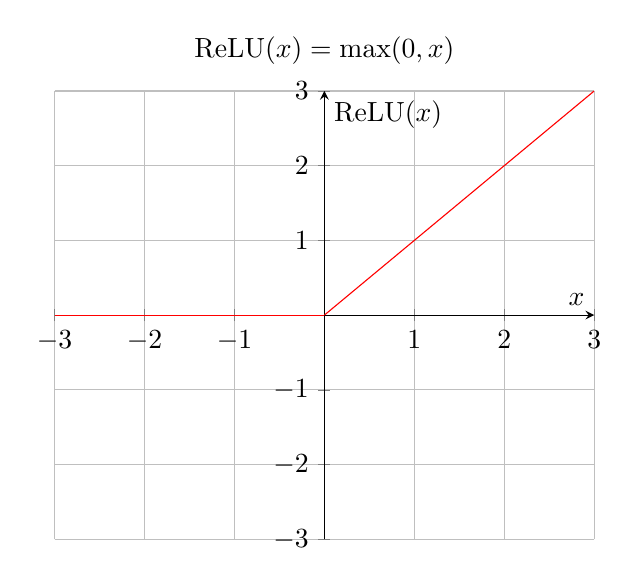
\begin{tikzpicture}
\begin{axis}[grid=major,
title={$\textup{ReLU}(x)=\textup{max}(0,x)$},
xlabel=$x$, ylabel=$\textup{ReLU}(x)$,ymin=-3, ymax=3,axis x line=middle,axis y line=middle,ytick={-3,-2,-1,0,1,2,3},]
% density of Normal distribution:
\addplot+[mark=none,red,domain=-3:0,] {0};
\addplot+[mark=none,red,domain=0:3,] {x};
\end{axis}
\end{tikzpicture}
% -- avoid white space
%
\hskip 20pt % insert a non-breaking space of specified width.
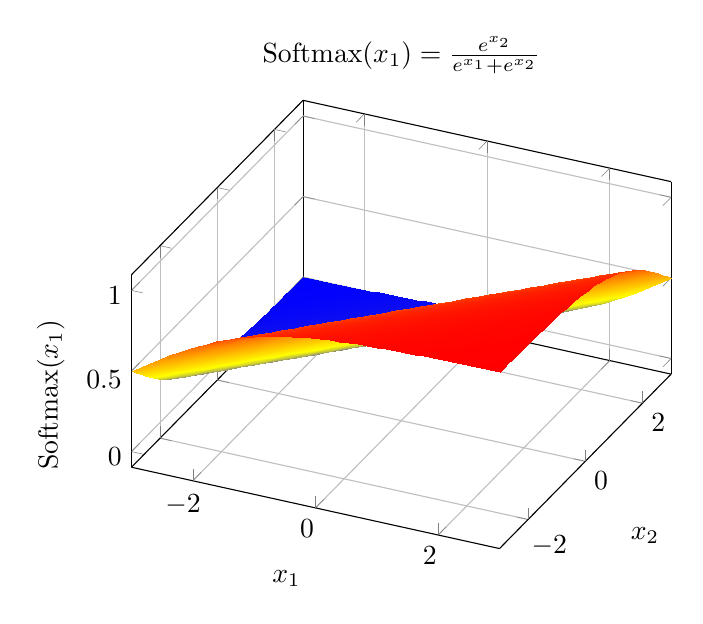
\begin{tikzpicture}
%\begin{axis}[
%title={$x \exp(-x^2-y^2)$},
%xlabel=$x$, ylabel=$y$,
%domain=-3:3,
%samples=201,
%]
\begin{axis}[grid=major,
title={$\textup{Softmax}(x_1)=\frac{e^{x_2}}{e^{x_1}+e^{x_2}}$},
xlabel=$x_1$, ylabel=$x_2$,zlabel=$\textup{Softmax}(x_1)$,view/v=45,]
\addplot3 [
surf,
shader=interp,
samples=40,
domain=-3:3,
y domain=-3:3,
small,
] {exp(x)/(exp(x)+exp(y))};
\end{axis}
\end{tikzpicture}
% -- avoid white space
%
\hskip 20pt % insert a non-breaking space of specified width.
%
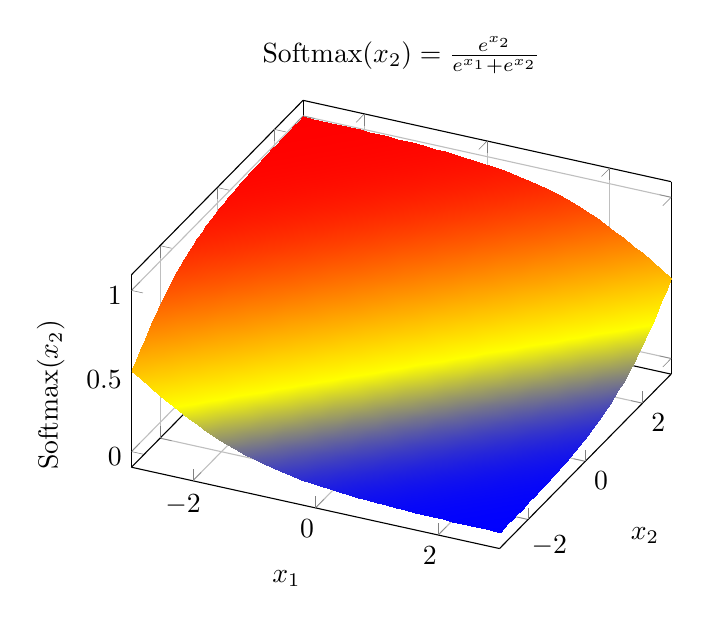
\begin{tikzpicture}
%\begin{axis}[
%title={$x \exp(-x^2-y^2)$},
%xlabel=$x$, ylabel=$y$,
%domain=-3:3,
%samples=201,
%]
\begin{axis}[grid=major,
title={$\textup{Softmax}(x_2)=\frac{e^{x_2}}{e^{x_1}+e^{x_2}}$},
xlabel=$x_1$, ylabel=$x_2$,zlabel=$\textup{Softmax}(x_2)$,view/v=45,]
\addplot3 [
surf,
shader=interp,
samples=40,
domain=-3:3,
y domain=-3:3,
small,
] {exp(y)/(exp(x)+exp(y))};
\end{axis}
\end{tikzpicture}
\hskip 20pt % insert a non-breaking space of specified width.
\end{document}
